\documentclass{standalone}
\usepackage{tkz-fct}
\usepackage{tkz-euclide}
\usepackage{amsmath}
\usepackage{color}
\renewcommand*\familydefault{\sfdefault}
\usepackage{sansmath}
\sansmath
\renewcommand{\arraystretch}{2.6}
\definecolor{gray75}{gray}{0.75}
\begin{document}

 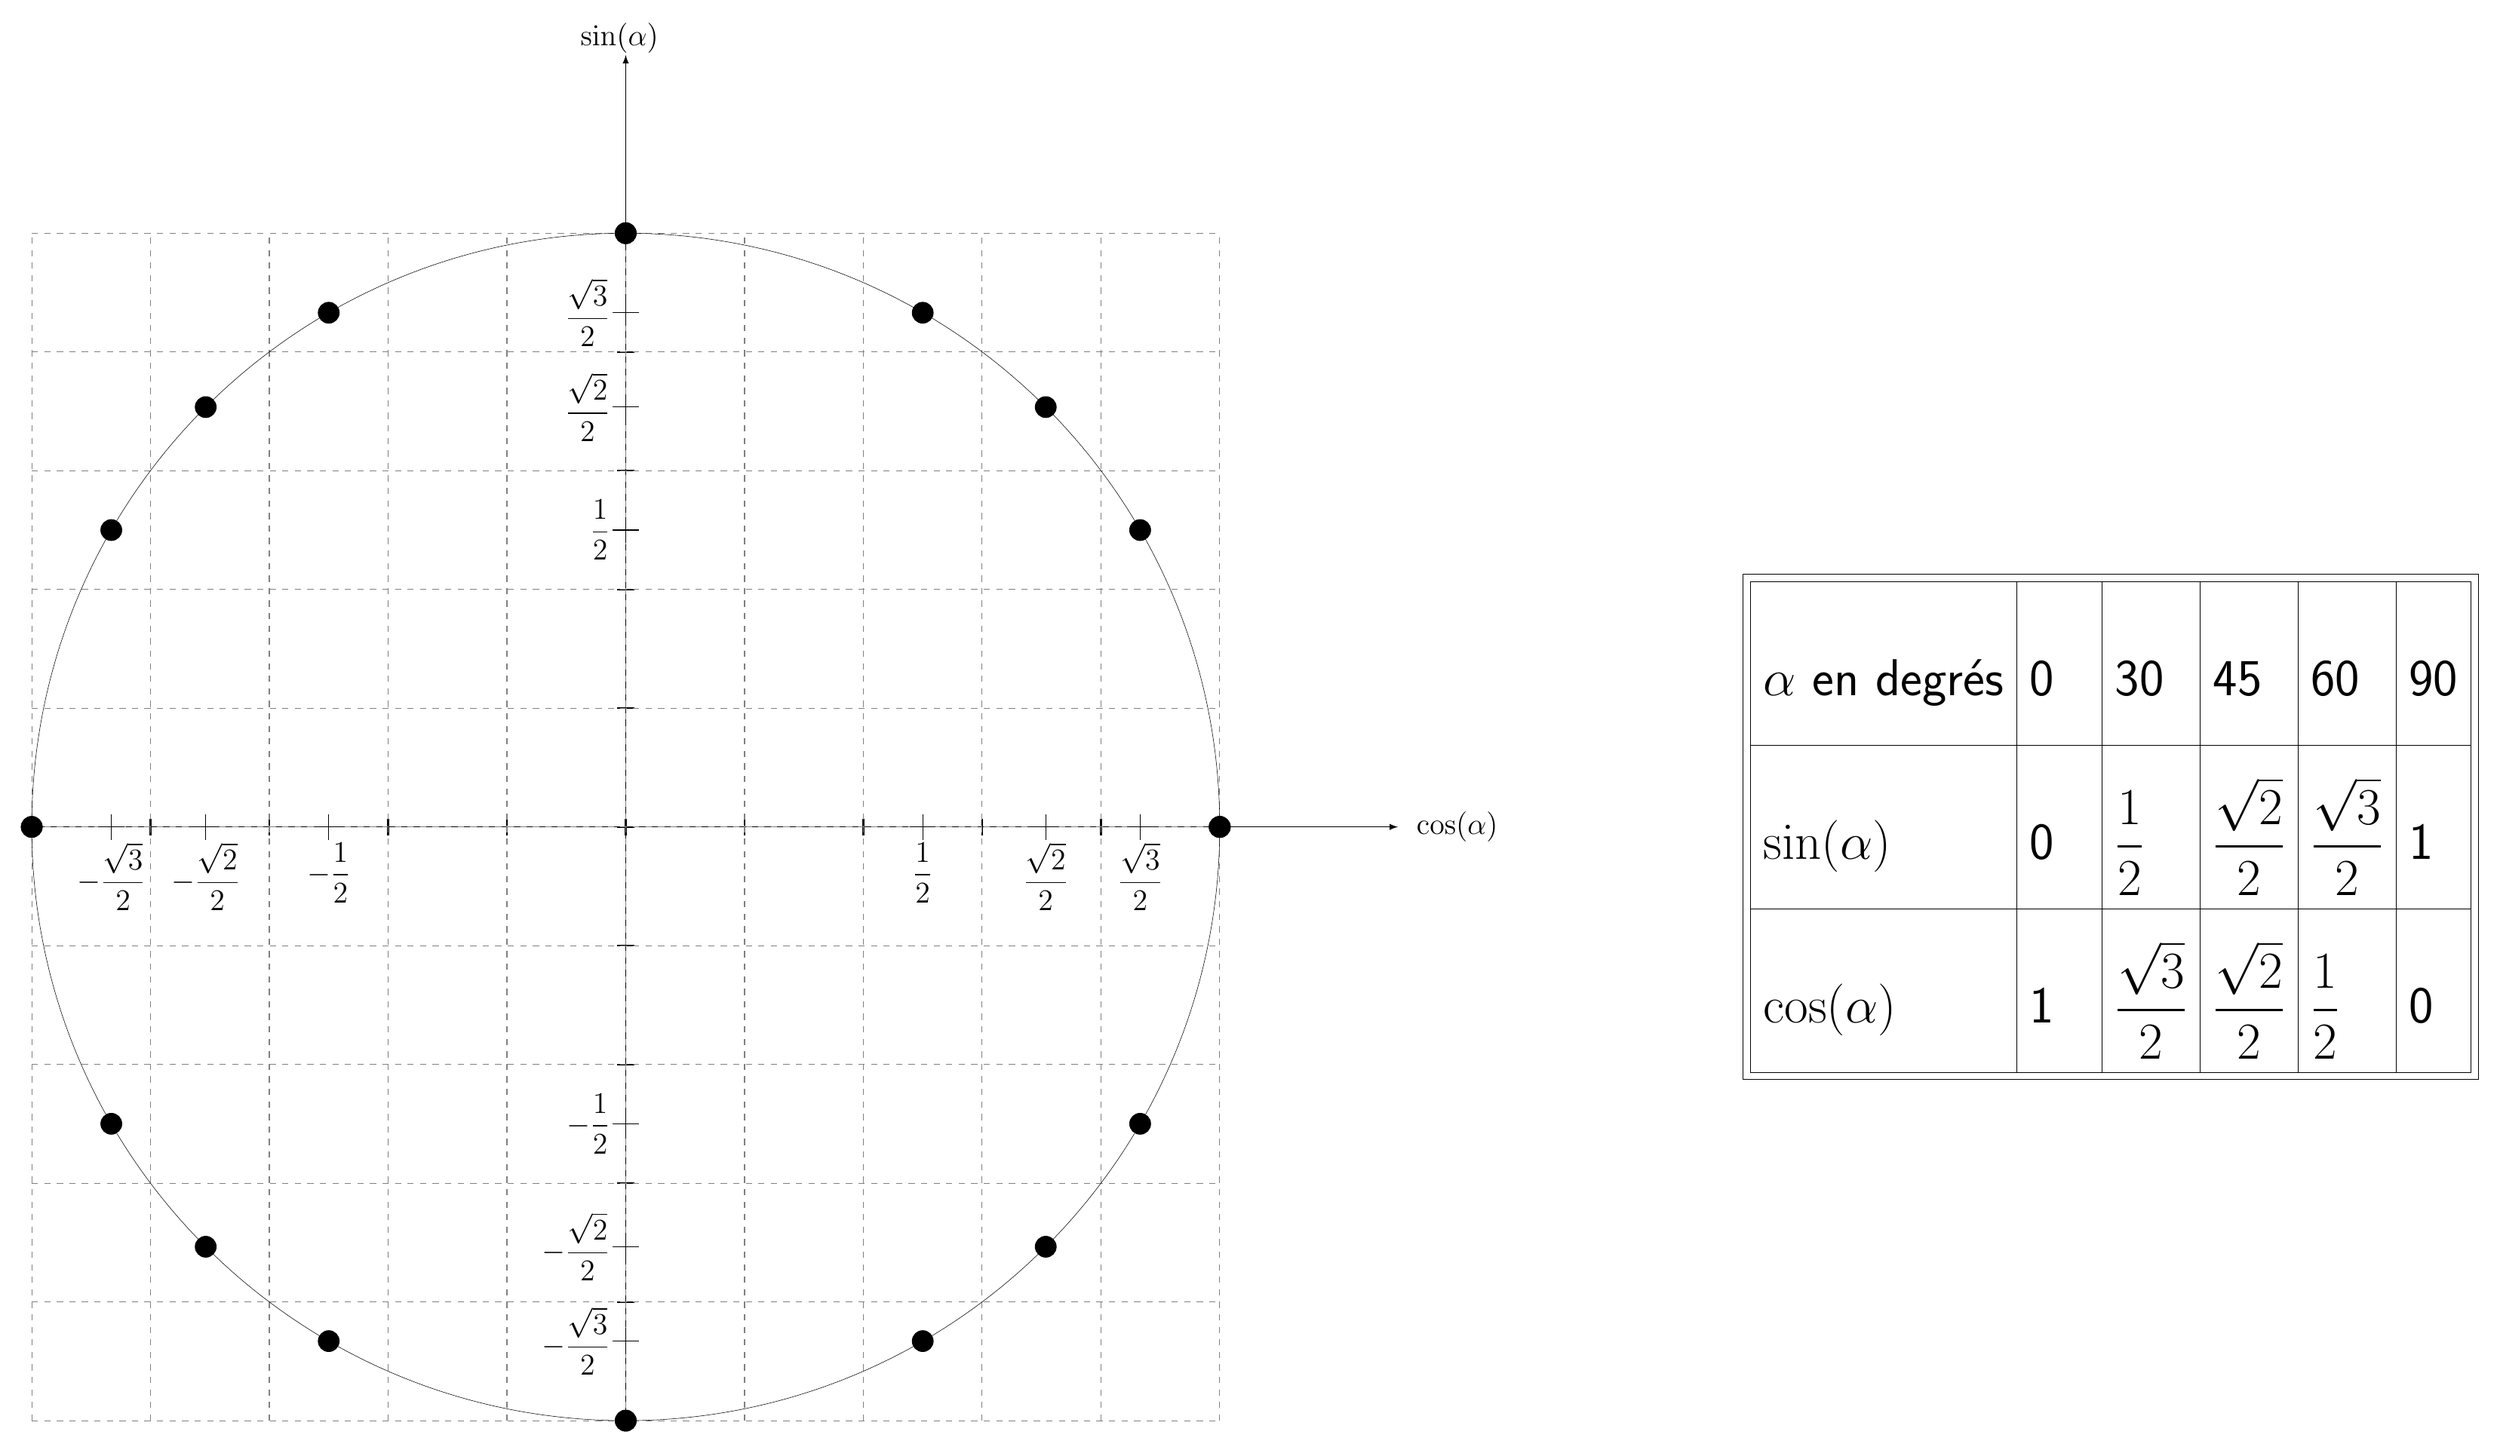
\begin{tikzpicture}[scale=2]
   \tkzInit[xmax=1.,ymax=1.,xmin=-1. ,ymin=-1,xstep=0.2,ystep=0.2]
     \tkzDrawY[label=$\sin(\alpha)$, above, font=\Large, up space=1.5]
   %\tkzLabelY[node font=\Large]
   %\tkzLabelX[node font=\Large]
   \tkzDrawX[label=$\cos(\alpha)$, right=8pt, font=\Large, right space=1.5]
   \begin{scope}[dashed]
     \tkzGrid
   \end{scope}

   \tkzDefPoints{0/0/O,1/0/A}

   \tkzDrawCircle[color=black](O,A)
   \foreach \a in {0,30,60,...,360}{%
     \tkzDefPointBy[rotation= center O angle \a](A)
     \tkzGetPoint{a}
     \tkzDrawPoint[size=10](a)
   }
   \foreach \a in {0,45,...,360}{%
     \tkzDefPointBy[rotation= center O angle \a](A)
     \tkzGetPoint{a}
     \tkzDrawPoint[size=10](a)
   }
   \tkzDefPoints{0/0.5/S1,0/0.70710678118/S2,0/0.86602540378/S3}
   \tkzDrawPoints[shape=cross,size=12](S1,S2,S3)
   \tkzLabelPoint[left=4pt](S1){\Large$\dfrac{1}{2}$}
   \tkzLabelPoint[left=4pt](S2){\Large$\dfrac{\sqrt{2}}{2}$}
   \tkzLabelPoint[left=4pt](S3){\Large$\dfrac{\sqrt{3}}{2}$}
      \tkzDefPoints{0/-0.5/S1,0/-0.70710678118/S2,0/-0.86602540378/S3}
   \tkzDrawPoints[shape=cross,size=12](S1,S2,S3)
   \tkzLabelPoint[left=4pt](S1){\Large$-\dfrac{1}{2}$}
   \tkzLabelPoint[left=4pt](S2){\Large$-\dfrac{\sqrt{2}}{2}$}
   \tkzLabelPoint[left=4pt](S3){\Large$-\dfrac{\sqrt{3}}{2}$}
   \tkzDefPoints{0.5/0/S1,0.70710678118/0/S2,0.86602540378/0/S3}
   \tkzDrawPoints[shape=cross,size=12](S1,S2,S3)
   \tkzLabelPoint[below=4pt](S1){\Large$\dfrac{1}{2}$}
   \tkzLabelPoint[below=4pt](S2){\Large$\dfrac{\sqrt{2}}{2}$}
   \tkzLabelPoint[below=4pt](S3){\Large$\dfrac{\sqrt{3}}{2}$}
      \tkzDefPoints{-0.5/0/S1,-0.70710678118/0/S2,-0.86602540378/0/S3}
   \tkzDrawPoints[shape=cross,size=12](S1,S2,S3)
   \tkzLabelPoint[below=4pt](S1){\Large$-\dfrac{1}{2}$}
   \tkzLabelPoint[below=4pt](S2){\Large$-\dfrac{\sqrt{2}}{2}$}
   \tkzLabelPoint[below=4pt](S3){\Large$-\dfrac{\sqrt{3}}{2}$}


     \tkzText[draw](2.5,0){\Huge
\begin{tabular}{|l|p{1cm}|l|l|l|l|}
\hline
$\alpha$ en degrés  & 0 & 30                    & 45                    & 60                    & 90               \\ \hline
$\sin(\alpha)$      & 0 & $\dfrac{1}{2}$        & $\dfrac{\sqrt{2}}{2}$ & $\dfrac{\sqrt{3}}{2}$ & 1                \\ \hline
$\cos(\alpha)$      & 1 & $\dfrac{\sqrt{3}}{2}$ & $\dfrac{\sqrt{2}}{2}$ & $\dfrac{1}{2}$        & 0                \\ \hline
\end{tabular}
     }
 \end{tikzpicture}

\end{document}
